\section{Introduction to \LaTeX}

\LaTeX, I had never heard about this term before doing this project,
but when I came to know about its features, found it excellent. 
\LaTeX{} (pronounced /ˈleɪtɛk/, /ˈleɪtɛx/, /ˈlɑːtɛx/, or /ˈlɑːtɛk/) is a 
document markup language and document preparation system for the \TeX{} 
typesetting  program. Within the typesetting system, its name is styled 
as \LaTeX.

\image{0.9}{images/donald.png}{Donald Knuth, Inventor Of \TeX{} 
typesetting system}

Within the typesetting system, its name is styled as \LaTeX. The term 
\LaTeX{} refers only to the language in which documents are written, 
not to the editor used to write those documents. In order to create a 
document in \LaTeX, a .tex file must be created using some form of text 
editor. While most text editors can be used to create a \LaTeX{} document, 
a number of editors have been created specifically for working with \LaTeX.

\LaTeX{} is most widely used by mathematicians, scientists, 
engineers, philosophers, linguists, economists and other scholars in 
academia. As a primary or intermediate format, e.g., translating DocBook 
and other XML-based formats to PDF, \LaTeX{} is used because of the 
high quality of typesetting achievable by \TeX. The typesetting system 
offers programmable desktop publishing features and extensive facilities 
for automating most aspects of typesetting and desktop publishing, 
including numbering and cross-referencing, tables and figures, 
page layout and bibliographies.

\LaTeX{} is intended to provide a high-level language that
accesses the power of \TeX. \LaTeX{} essentially comprises a
collection of \TeX{} macros and a program to process \LaTeX documents. 
Because the \TeX{} formatting commands are very low-level, it is usually 
much simpler for end-users to use \LaTeX{}.


\subsection{Typesetting}
\LaTeX{} is based on the idea that authors should be able to focus on 
the content of what they are writing without being distracted by its 
visual presentation. In preparing a \LaTeX{} document, the author 
specifies the logical structure using familiar concepts such as 
chapter, section, table, figure, etc., and lets the \LaTeX{} system 
worry about the presentation of these structures. It therefore 
encourages the separation of layout from content while still allowing 
manual typesetting adjustments where needed. 

\begin{verbatim}
\documentclass[12pt]{article}
\usepackage{amsmath}
\title{\LaTeX}
\date{}
\begin{document}
  \maketitle 
  \LaTeX{} is a document preparation system 
  for the \TeX{} typesetting program.
   \par 
   $E=mc^2$
\end{document}
\end{verbatim}
\image{0.3}{images/latexoutput.png}{\LaTeX{} output of above program.}

\subsection{Installing \LaTeX{} on System}
Installation of \LaTeX{} on personal system is quite easy. As i have used \LaTeX{} on Ubuntu 13.04 so i am discussing the installation steps for Ubuntu 13.04 here:
\begin{itemize}
\item Go to terminal and type\\\\
\textit{\$ sudo apt-get install texlive-full}
\item Your Latex will be installed on your system and you can check for manual page by typing.\\\\
\textit{\$ man latex}\\
in terminal which gives manual for latex command.\\
\item To do very next step now one should stick this to mind that the document which one is going to produce is written in any type of editor whether it may be your most common usable editor Gedit or you can use vim by installing first vim into your system using command.\\\\
\textit{\$ sudo apt-get install vim}\\
\item After you have written your document it is to be embedded with some set of commands that Latex uses so as to give a structure to your document. Note that whenever you wish your document to be looked into some other style just change these set of commands.\\\\
\item When you have done all these things save your piece of code with .tex format say test.tex. Go to terminal and type\\\\
\textit{latex path of the file test.tex Or pdflatex path of the file test.tex\\ eg: pdflatex test.tex}\\
for producing pdf file simultaneously.\\
After compiling it type command\\\\
\textit{\$ evince filename.pdf\\ eg: evince test.pdf}\\
To see output pdf file. 
\end{itemize}

\subsection{Graphical Editors for \LaTeX{}}
\LaTeX{} is not restricted to command line only there are so many graphical based editors available to be used. These GUi based editors provide an easy interface to user so as to do typesetting in an efficient manner. Some of them are listed below:
\begin{itemize}
\item {Texmaker}
\begin{figure}[ht]
\centering
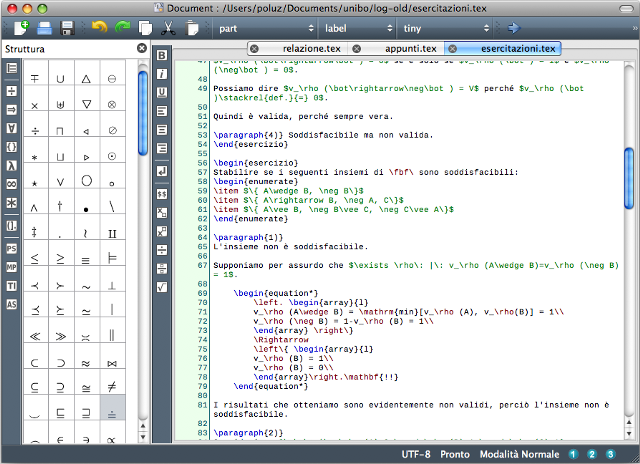
\includegraphics[scale=0.4]{images/texmaker.png}
\caption{Texmaker, A Graphical \LaTeX{} Editor}
\end{figure}
\item LEd
\begin{figure}[ht]
\centering
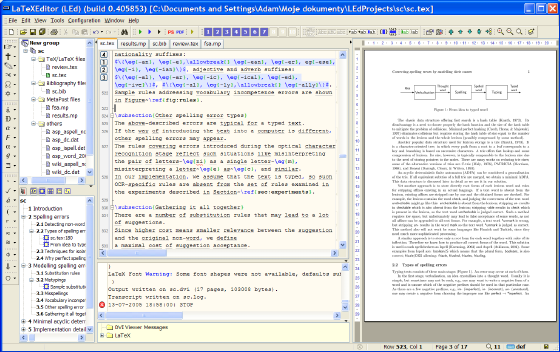
\includegraphics[scale=0.5]{images/led.png}
\caption{LEd, A Graphical \LaTeX{} Editor}
\end{figure}
\end{itemize}
And many more but the preferred method to produce \LaTeX{} document is through console mode only.


\subsection{Pdfscreen \LaTeX{}}
There are some packages that can help to have unified document using \LaTeX{}. Example of such a package is pdfscreen that let the user view it’s document in two forms-print and screen. Print for hard copy and screen for viewing your document on screen. Download this package from www.ctan.org/tex-archive/macros/latex/contrib/pdfscreen/.\\
Then install it using above mention method.\\

Just changing print to screen gives an entirely different view. But for working of pdfscreen another package required are comment and fancybox.\\

The fancybox package provides several different styles of boxes for framing and rotating content in your document. Fancybox provides commands that produce square-cornered boxes with single or double lines, boxes with shadows, and round-cornered boxes with normal or bold lines. You can box mathematics, floats, center, flushleft, and flushright, lists, and pages.\\

Whereas comments package selectively include/excludes portions of text. The comment package allows you to declare areas of a document to be included or excluded. One need to make these declarations in the preamble of your file. The package uses a method for exclusion that is pretty robust, and can cope with ill-formed bunches of text.\\

So these extra packages needed to be installed on system for the proper working of pdfscreen package.
\subsection{Web based graphic generation using \LaTeX{}}
\LaTeX{} is also useful when there is need of generating the graphics from browser. For
example to draw a circle by just entering its radius in html input box. So this kind
A
of project can be conveniently handled using \LaTeX{}. Basic idea behind this generation
process is that when user clicks on submit button after entering radius a script will run
that enter the radius in already made .tex file and recompiles it on server and makes its
pdf and postscript file. After that user can view those files by clicking on link provided
to view the files. See some screen shots of such a graphic generation project made by
Dr. H.S. Rai:\\

So here in the above input page which is also the index page user can enter input
for length of rectangle, breadth of rectangle and for radius of circle after that user can submit the values. After the values get submitted a script get runs by php code at server
side. This script first enters the dimensions of rectangle and circle that were selected by
user in to an already existing .tex file and replace with the older dimensions there. After
that script recompiles the the tex file and make it available for user.\\

In above figure it gets clear that .tex file has been compiled and pdf and postscript files
are available to user and user can download the graphics so produced. Hence graphics
can be generated in \LaTeX{} through web interface.
\begin{figure}[ht]
\centering
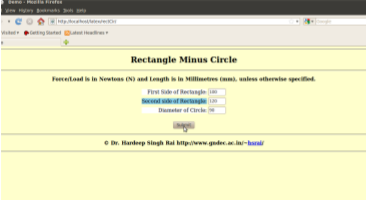
\includegraphics[scale=0.5]{images/webgraphic.png}
\caption{Web based graphic generation using \LaTeX{}(input page)}
\end{figure}
